\documentclass{article}

\usepackage{amsmath}
\usepackage{graphicx}

\begin{document}

\section{Measurement setup}

Our measurement setup consists of 3 main parts:
\begin{itemize}
    \item An endrun ninja ptp grandmaster clock synchronized via GPS.
    \item A raspberry pi 4 compute module with an Intel i210 NIC
    \item A Basys-3 FPGA development board setup to measure pps pulses.
\end{itemize}

The ptp grandmaster is connected via a direct ethernet cable to the i210 nic, and this connection is used to carry the PTP messages. Both the ptp grandmaster and the intel nic are configured to produce pulse-per-second outputs. Furthermore, the raspberry pi is also configured to produce a pulse-per-second output on its gpio pins.

All these pulses are measured by the FPGA relative to its internal clock. Although this internal clock is not precise, we can estimate its frequency using the pulse-per-second signal from the ptp grandmaster.

The grandmaster configuration is the default provided by endrun, and the grandmaster is given time to fully lock onto the GPS signal before start of measurement (specifically, we wait until the clock quality reported by gpsstat is at level 3).

On the raspberry pi, depending on the run we either start the linuxptp stack or statime. We then wait with starting the measurement until the self-reported offset to the grandmaster appears stable.

\section{Error estimates}

In our analysis we will include the following 4 main error sources: Cable length differences, fpga input path differences, discretization error, and fpga clock instability. Below we will discuss each, including their contributions to our estimated error.
\subsection{Cable length}
The setup contains cables of multiple lengths and varying electrical characteristics. We will estimate these errors pessimistically and assume maximum systematic errors up to the propagation delay of our longest possible cable. As all our cables are below 1.5 meters in length, this gives us an estimated 15ns of systematic error.
\subsection{FPGA input architecture}
Although care has been taken in the VHDL code the fpga has been programmed with to keep the input path for all of the signals identical, due to the fact that these interact with different pieces of the physical hardware there can still be offsets between processing delays for the inputs. Based on the documentation of the FPGA's architecture, we assume these to contribute 1 fpga clock cycle of systematic error.
\subsection{Discretization error}
The pulse per second signals arrive at the fpga unsynchronized with the fpga's clock. Due to this, their measured arrival time may be off by up to 1 clock cycle, giving us a statistical error of 1 fpga clock cycle.
\subsection{FPGA clock instability}
The clock in the fpga is of relatively low quality, and may therefore be somewhat unstable. We will use the pulse-per-second signal measured from the grandmaster clock to estimate the frequency instability of the fpga's clock, which will provide us with an additional statistical error component.

\section{FPGA clock callibration}

We callibrate the FPGA clock using the data from the GM pulse-per-second signal. Note that this process purely uses difference between arrival times of these pulses, hence errors from cable length can be ignored in the following analysis.

\begin{figure}[h]
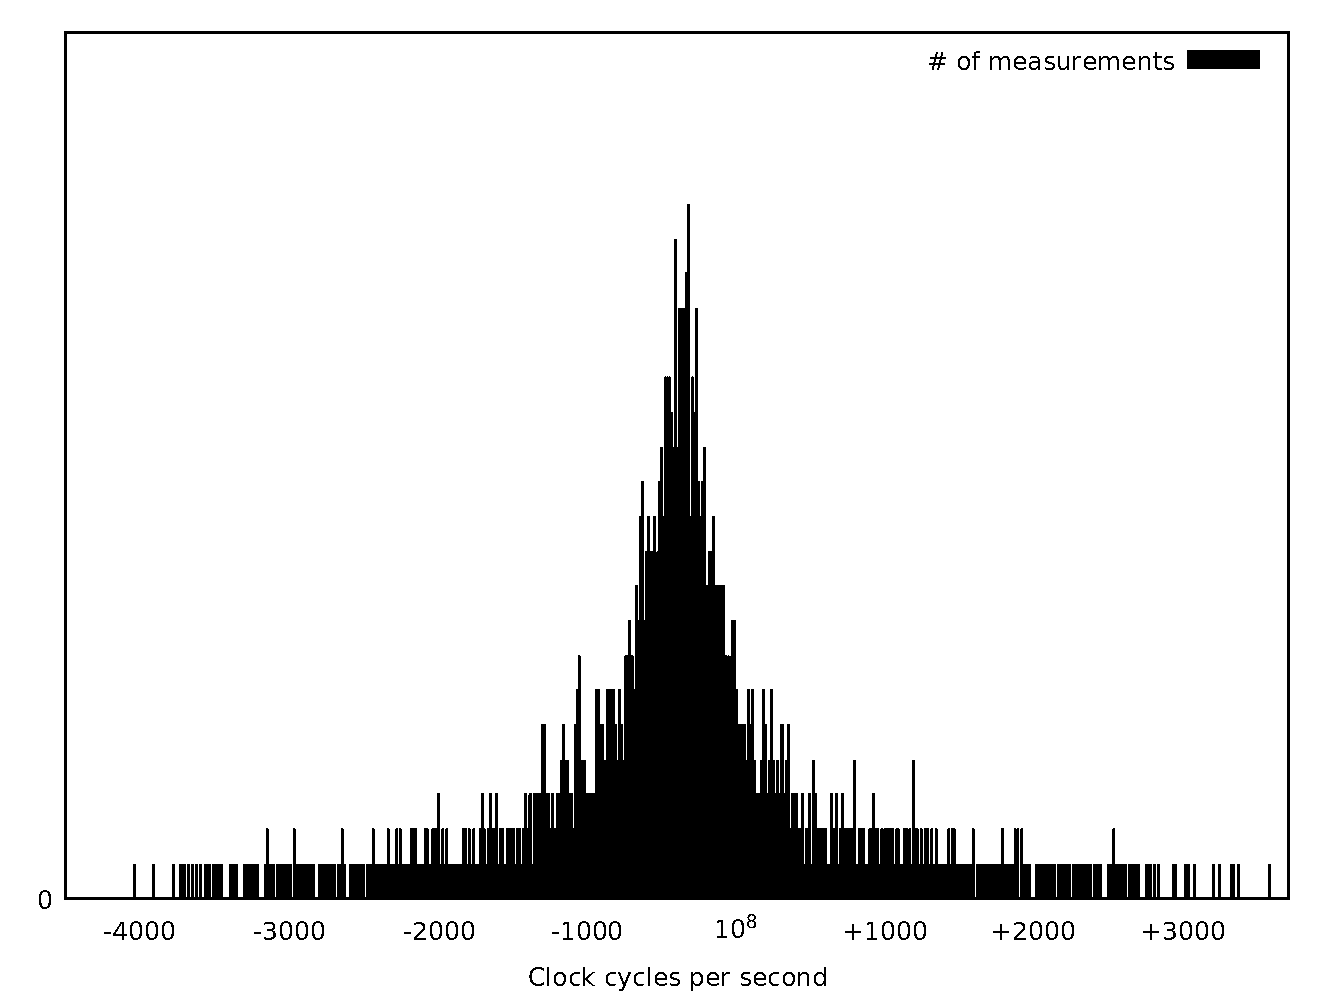
\includegraphics[width=0.5\textwidth]{gm_clocks_per_sec_ref.pdf}
\caption{FPGA clock cycles per second as measured using the GM pulse-per-second output. On the left is data from the linuxptp run, from the right from the statime run.}
\label{fig:gm_cycles_per_second}
\end{figure}

For the linuxptp run, the measurement data are plotted in Figure~\ref{fig:gm_cycles_per_second}. Analysing this shows that 1 second takes $9.99996\cdot 10^7 \pm 7.5\cdot 10^2 (\text{stat}) \pm 0.01\cdot 10^2 (\text{sys})$ cycles. This gives us an estimated clock period of $10.0000370 \pm 7.5\cdot 10^{-5} (\text{stat}) \pm 0.01\cdot 10^{-5} (\text{sys})$ nanoseconds.

\end{document}